% !TEX root = ../../book.tex

\chapter{Algorithmic Trading In Electronic Platforms}

While algorithmic trading techniques are useful in both low and high frequency settings, their importance has become more pronounced in the age of electronic trading because of the speed in execution and the necessity for efficient matching of demand and supply sides in the limit order books. Added to this is that modern equity markets where order submission and cancellations are automated are also highly fragmented with dozens of exchanges and about forty alternative trading systems where investors can choose to trade. The trading algorithms differ over various types of market participants, but all of them try to optimize dynamically where, how often and at what price to trade. Typically, the execution layers can be broadly described as follows (see Gatheral (2012)\cite{}):
	\begin{itemize}
	\item \textbf{The Macrotrader:} Given a meta-order (parent trade) translate the objective function of a strategy into a trading schedule; when the algorithm should trade, in what size (child order) and for how long.
	\item \textbf{The Microtrader:} Given a slice (child order) of the meta-order to trade, this layer of algorithm decides whether to place it as a market or as a  limit order and at what price level.
	\item \textbf{The Smart Order Router:} For a given order (quantity and price level) to which venue should the order be sent.
	\end{itemize}


In this chapter we discuss these and other execution issues in the high frequency trading context. Generally the objectives of equity trading are to minimize the probability of making errors--minimizing the trading impact and avoiding adverse selection. In order to achieve high completion rates, the trading should operate with speed and necessary risk control. It has to be noted that the average trade size has come down over time; thus the parent order are increasingly decimated and are sent to the exchanges as small child orders. Handling this with large parent order sizes with the focus on short-term alphas requires a great deal of trade timing insights.  


\section{Execution Algorithms:  History and Review}


The primary goal of most of the execution algorithms is to minimize the transaction costs which are broadly divided into direct costs and into indirect costs. The direct costs such as commissions, taxes etc are easy to measure and primarily depend on quantity of trading. The indirect costs such as market impact and opportunity costs are hard to measure and depend upon trading strategies. Because many mutual fund and hedge fund companies engage in portfolio rebalancing periodically, they trade a large block of shares in a fixed duration. There is a trade-off between trading a large market order that is likely to affect the price adversely and splitting the parent order into many child orders and let the market recover after each trade. The modeling elements generally involve representing the permanent impact of a parent order and the temporary impact of trading a child order when the price normally returns back to equilibrium, short time after the trade, drift in price (alpha) and the volatility of the stock. The optimizing function balances the cost-loss in revenue due to price impact and the risk-uncertainty due to volatility of the underlying stock. If the trade occurs fast, we incur high cost and low risk but if the trade is slow, we incur low cost and high risk.


The execution algorithms are generally evaluated through some benchmark prices. Some examples are:
	\begin{enumerate}[--]
	\item $p_0$: Arrival price, that is the market mid-quote at the start of parent order execution at $t=0$.
	
	\item $p_{\text{VWAP}}$: Volume weighted average market price over the period of execution, $t \in (0,T)$. \\
	
	If the parent order of size, $X$ is split into `$n$' child orders with size, $x_k$, $k=1,\ldots,n$, then
	
	\item $p_{\text{exec}}$: Volume weighted average price of the parent order's execution. \\
	
	Two related quantities that the traders examine in their evaluation strategies are
	
	\item $p_{\text{bench}}-p_{\text{exec}}$: Slippage$=x$;
	
	\item $p_0-p_{\text{VWAP}}$: Market Impact 
	\end{enumerate}
	
The execution cost is taken to be the slippage and the execution risk is its standard deviation. 


The influential paper by Kyle (1985)~\cite{kyle1985} argues that traders split the parent order to hide private information. The splitting of the order and how they are sent to the market--the strategies--depend on the evolution of the stock price. These are broadly classified into static, one determined in advance of trading and into dynamic, one that depends on the state of the market. The static strategy under some conditions can also be dynamically optimal. Few commonly used strategies are: \\

VWAP-Strategy: $x_k=x \cdot \dfrac{V_k}{V}$ \\

Implementation Shortfall Strategy: Minimize $E(x)+\lambda \Var(x)$ \\

Percentage of Volume Strategy: Minimize $\left(\dfrac{\text{Volume}_{\text{exec}}}{\text{Volume}_{\text{market}}} - v_{\text{target}}\right).$ \\

\noindent These strategies are static and they are based on a priori models for the evolution price and volume traded over different times of the day. 


We present below select results in this area. The quantities that the trader can determine are the number of child orders $(n)$ and their sizes $(x_k)$ and the duration for the trading $(T)$. The relevance of this problem to the practitioners is discussed in Chan and Lakonishok (1997)~\cite{lakon} and Keim and Madhavan (1997)~\cite{madhavan}. Bestimas and Lo (1998)~\cite{berlo} develop a model that suggests splitting the parent order to reduce the average trading costs. Almgren and Chriss (2000)~\cite{alm2000} split the parent order to minimize the mean-variance of trading costs similar to Markowitz's portfolio theorem. We describe in the following sections, these strategies which are mainly static. 


\subsection{Bertsimas and Lo Model}


The basis of the model discussed here is that trading affects not only the current prices but also the price dynamics that affects the future trading costs. Thus the problem involves dynamic optimization but the solution turns out to be static. Assume that an investor wants to sell a parent order of $X$-shares in $(0,T)$, where $T$ is arbitrary, and let $x_k$ be the number of shares sold (child orders) with the realized price, $\widetilde{p}_k$. The cost of trading, also know as slippage is:
	\begin{equation}\label{eqn:x7}
	x = Xp_0 - \sum_{k=1}^n x_k\widetilde{p}_k
	\end{equation}
where $p_0$ is the arrival price. The model proposed in Bertsimas and Lo (1998)~\cite{berlo} can be stated as:
	\begin{equation}\label{eqn:xk7}
	\min_{x_k} E_1 \left[\sum_{k=1}^n x_kp_k\right] \text{ such that }\sum_{k=1}^n x_k=X
	\end{equation}
The criteria in (\ref{eqn:xk7}) call for determining the sizes of child orders a priori. To solve (\ref{eqn:xk7}), the model for price, where the price impact and price dynamics are separated, is taken to be,
	\begin{equation}\label{eqn:pk7}
	p_k = p_{k-1} - \theta x_k + \varepsilon_k
	\end{equation}
where $\theta > 0$ representing the price impact and when $\theta = 0$, the model is simply a random walk model discussed in Chapter 2. Under (\ref{eqn:pk7}) the best strategy for splitting the parent order, $x$, is shown to be
	\begin{equation}\label{eqn:equals}
	x_1^* = x_2^* =...= x_n^* = \frac{X}{n}
	\end{equation}
the equal split. What the trader needs to decide a priori is the number of splits, $n$. The allocation strategy in (\ref{eqn:equals}) is termed as the time weighted average prices (TWAP) strategy in industry. 


The dynamic programming solution to (\ref{eqn:xk7}) via the so called Bellmann equation is elegant and simple because the price impact $(\theta x_k)$ does not depend upon the prevailing price $(p_{k-1})$ nor on the size of the unexecuted order $(X - \sum_{j=1}^{k-1} x_j)$. The indirect assumptions here are that the volume curve is even over different times of the day and the volatility profile are flat. Bestimas and Lo (1998)~\cite{berlo} also consider extensions of the model (\ref{eqn:pk7}), where a serially correlated state variable such as market condition (S\&P 500) is added. In this case it is shown that the best execution strategy at any point is a function of the state variable and the remaining unexecuted size. 


As a point of comparison to the equal allocation strategy observe that VWAP-strategy is similar in the sense that is does not also depend on any price movement. Simply the allocation is made as $\frac{x_k}{X}=\frac{V_k}{V}$, which leads to
	\begin{equation}\label{eqn:xk}
	x_k = X \dfrac{V_k}{V}
	\end{equation}
where $V_k$ is the market volume during the $k$th time interval. If the traders are restricted to only `$n$' time intervals, it is important to have a good forecast for the quantities, $V_k$ and thus, $V$. 


\subsection{Almgren and Chriss Model}


The seminal paper by Almgren and Chriss (2000)~\cite{alm2000} and Almgren (2003)~\cite{} consider the same problem taking into account the stock characteristics such as volatility via the mean-variance formulation of minimizing execution costs. The formulation treats the execution as a tradeoff between risk and cost; the faster the execution, higher the cost but lower the risk. The objective again is to liquidate, $X$ units before time `$T$' at minimum cost, in time steps, $t_k = k\tau$ for $k = 0,1,\ldots, n$ where $\tau = T/n$ is the average length of interval between successive child order submission times. If $X_k$ is the number of units held at $t_k$, the goal is to decide on the trading trajectory, $X_0,X_1,\ldots,X_n$ with $X_0=X$ and $X_n=0$. The number of units liquidated $x_k$ between $t_{k-1}$ and $t_k$ is called the trading schedule, with $x_k = X_{k-1} - X_k$. The trading strategy requires determining `$x_k$' in terms of information available at $t_{k-1}$. The static strategies determine the trading schedule in advance of starting trade time, $t_0$ and the dynamic strategies depend on information available up to $t_{k-1}$. Almgren and Chriss (2000)~\cite{alm2000} find trading trajectories that minimize $E(x)+\lambda \Var(x)$ for various values of $\lambda$.


The model for price impact is same as in (\ref{eqn:pk7}) but stated as
	\begin{equation}\label{eqn:bigpk}
	p_k=p_{k-1} - (\tau\theta)\dfrac{x_k}{\tau} + \sigma\tau^{1/2}\varepsilon_k
	\end{equation}
where $v_k = x_k/\tau$ is the average rate of trading in $[t_{k-1}, t_k]$ and $\varepsilon_k$ are independent with mean zero and unit variance and `$\sigma$' is the volatility of the stock. The temporary impact represented by price per share received for sale in $[t_{k-1}, t_k]$ is
	\begin{equation}\label{eqn:pdouble}
	\begin{split}
	\widetilde{p}_k &= p_{k-1} - \eta\left(\dfrac{x_k}{\tau}\right) \\
			&= p_{k-1} - c \sgn(x_k) + \frac{\eta}{\tau}\cdot x_k
	\end{split}
	\end{equation}
where $c$ can be taken to be fixed cost of selling which is the sum of mid-spread and fees. The temporary impact component is not present in the next period. Note (\ref{eqn:xk}) can be written as,
	\begin{equation}\label{eqn:morepk}
	p_k = p_0 + \sigma\tau^{\frac{1}{2}}\sum_{j=1}^k\varepsilon_j - \theta(X - X_k)
	\end{equation}
and thus the shortfall,
	\begin{equation}\label{eqn:longxeq}
	x = Xp_0 - \sum_{k=1}^N x_k\widetilde{p}_k = \sum_{k=1}^N \left(\frac{x_k}{\tau}\right) \eta - \sum_{k=1}^N \,[\sigma\tau^{1/2}\varepsilon_k - \theta x_k]X_k
	\end{equation}
is a function of the market volatility and the trade schedule, `$x_k$'. It captures the difference between the initial book value and the weighted average of realized prices. From (\ref{eqn:longxeq}) it follows that
	\begin{equation}\label{eqn:evardouble}
	\begin{split}
	E(x) &=  \theta\sum_{k=1}^N x_k X_k + \eta\sum_{k=1}^N (\frac{x_k}{\tau}) \\
	\Var(x) &= \sigma^2\sum_{k=1}^N \tau X_{k}^2\cdot
	\end{split}
	\end{equation}
If the trajectory is to sell at a constant rate, $x_k = \frac{X}{n}$ and $X_k = (n - k)\frac{X}{n}$, $k = 1,\ldots,N$,
	\begin{equation}\label{eqn:secondevardouble}
	\begin{split}
	E(x) &= \frac{1}{2}\theta X^2 + \varepsilon X + \left(\eta - \frac{1}{2}\theta\tau\right)\frac{X^2}{T} \\
	\Var(x) &= \frac{1}{3}\sigma^2X^2T(1 - \frac{1}{N})(1-\frac{1}{2N})
	\end{split}
	\end{equation}
The trajectory minimizes expected cost but variance increases with $T$. On the other hand if we liquidate entire $X$ in the first time period,
	\begin{equation}\label{eqn:anotherdoubleex}
	\begin{split}
	E(x) &= c X + \eta \frac{X^2}{\tau} \\
	\Var(x) &= 0
	\end{split}
	\end{equation}
If $n$ is large, hence $\tau$ small, $E(x)$ can be very large significant resulting in impact price.


 With these illustrations of extremes, the optimization problem can be restated as,
	\begin{equation}\label{eqn:minex}
	\min_x (E(x) + \lambda V(x)) 
	\end{equation}
and if $\lambda>0$, $E(x)+\lambda V(x)$ is strictly convex and thus has a unique solution. The solution to (\ref{eqn:minex}) can be written as a combination of the exponentials. The results of trading trajectory and the trade list are given below:
	\begin{equation}\label{eqn:doublex}
	\begin{split}
	X_j &= \dfrac{\sinh (\kappa(T-t_j))}{\sinh (\kappa(T))}\cdot X, \enskip j=0,\ldots,N \\
	x_j &= \dfrac{2 \sinh (\frac{1}{2}\kappa\tau)}{\sinh (\kappa(T))}\cdot \cosh(\kappa(T-t_{j-\frac{1}{2}}))X, \enskip j=1,\ldots,n
	\end{split}
	\end{equation}
Here $t_{j-\frac{1}{2}} = (j - \frac{1}{2})\tau$ and $\kappa = \sqrt{\lambda\sigma^2/\eta}$, that depends on the volatility and the risk aversion coefficient, `$\lambda$' is termed as urgency parameter. The inverse of `$\kappa$' is termed as the trade's, ``half-life''; the larger its value the more rapid the depletion rate of the trade list. The solution given in (\ref{eqn:doublex}) is shown to be adaptive at any point in time, `$j$'. Thus the initial optimal solution over the entire interval is also optimal over each subinterval. A fixed trajectory as in (\ref{eqn:doublex}) was previously constructed by Grinold and Kahn (2000)~\cite{grin2000}.


The value of `$\lambda$', the price of risk depends on the traders utility function. The suggested optimal strategy is just volume weighted average pricing (VWAP), that is trading at a constant rate, when $\lambda \to 0$, that is if the trader is risk-neutral. The trade schedule for various value of `$\lambda$' is given in Figure~\ref{fig:7first} and the projected execution schedule is given in Figure~\ref{fig:7second}. Various extensions of the basic model (\ref{eqn:bigpk}) are considered by Almgren (2008)~\cite{alm2008}.
	\begin{figure}[!ht]
   	\centering
	    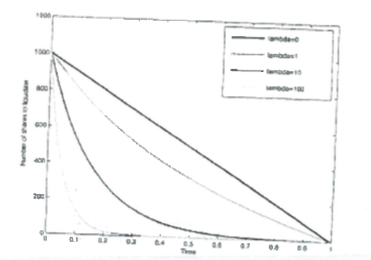
\includegraphics[width=\textwidth]{chapters/chapter7/figures/temp1.png}
	   \caption{Trade Schedule: The cross validation errors of lasso models with different levels of interactions. \label{fig:7first}}
	\end{figure}
	\begin{figure}[!ht]
	   \centering
	    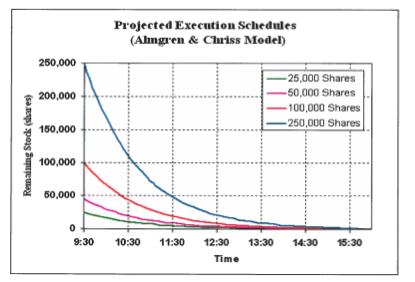
\includegraphics[width=\textwidth]{chapters/chapter7/figures/temp2.png}
	   \caption{Projected Execution Schedules \label{fig:7second}}
	\end{figure}
The effect of a short term drift in prices and the serial correlation in the errors which is observed in high frequency etc can be incorporated easily in the model (\ref{eqn:morepk}). Lorenz and Almgren (2011) \cite{lovenz2011} provide a Bayesian approach to the optimization problem. While the methodology yields elegant solutions, empirical use of these results require a close monitoring of order book dynamics as the changes in demand and supply sides are quite rapid.


The above mean-variance formulation of execution cost is combined with the traditional mean-variance portfolio optimization is Engle and Ferstenberg (2007)~\cite{engle2007} and Engle, Ferstenberg and Russell (2012)~\cite{engle2012}. We will discuss this in the context of portfolio rebalancing and the need for minimizing the transaction costs associated with all trades. 


\subsection{Obizhaeva and Wang Model}


The models discussed in the previous sections assume price impact function that is not sensitive to liquidity dynamics. Obizhaeva and Wang (2013)~\cite{obizhaeva} develop a model that accounts for the dynamic properties of supply and demand as represented in the limit order book. The model captures `resilience'; that is, how the current trade affects the status of the future limit order book. The resulting strategy consists of a large trade initially aimed at moving the order book away from its steady state followed by a number of small trades that will utilize the inflow of new liquidity providers. The speed at which the book replenishes itself is an important part of execution cost. The level of resilience depends on the level of hidden liquidity in the market. The price impact model considered here takes into account the dynamics of the limit order book.


It is assumed that the parent order $X$ will be traded in the interval $(0,T)$, `$n$' times at $t_1,t_2,\ldots,t_n$. To model the execution of a large order in the limit order book, it is assumed that the price of execution ($p_t$) depends on the true value of the equity ($p_t^*$) and the state umicsles ($z_t$) such as past trades that may affect the book. Let $q(p_t^*,P_t;z_t)$ be the density of the limit orders in the other side of the book. The mid-quote ($V_t$) is generally taken to reflect the true price, $p_t^*$. If the trade is on the buy side, the initial large transaction, $x_1$, can push the ask price to a higher level, $p_1^*+(s/2)+(x_1/q)$, where `$s$' is the spread and the average execution price is then equal to $p_1^*+(s/2)+x_1/(2q)$. After the initial execution the price converges to a new steady state, $p_t^*+s/2+\lambda x_1$. Assuming that the limit-order book converges to its steady-state exponentially and at time `$t$', 
	\begin{flalign}\label{eqn:qtdouble}
	&& q_t(p)&= q\cdot I(p>A_t) && \notag \\
	\text{and} && \phantom{x} & \phantom{x} && \\
	&& A_t&=V_t+\dfrac{s}{2}+x_1 \cdot \kappa e^{-\rho t} && \notag
	\end{flalign}
where $A_t$ is the asking price, $\kappa=1/q-\lambda$ and `$\rho$' measures the resilience of the limit order book. If more the current ask price ($A_t$) deviates from steady state level, $V_t+s/2$, the new ask limit orders will come into the book as the rate of $\rho \,q (A_t-V_t-s/2)$. 


Given the above description of the limit order book dynamics, the optimal execution problem can be restated as follows:
	\begin{equation}\label{eqn:min}
	\min_{x_k} E_1\left(\sum_{k=1}^n [A_k + x_k(2q)]x_k\right)
	\end{equation}
such that 
	\[
	A_k=p_k^*+\lambda(X_1-X_n)+\dfrac{s}{2}+\sum_{i=1}^{k-1} x_i\cdot \kappa e^{- \rho\tau(n-i)}
	\]
where $p_k^*$, the true price is taken to follow a random walk.


The solution to this dynamic programming problem is given in Obizhaeva and Wang (2013, p.14, Proposition 1)~\cite{obizhaeva} and is somewhat involved. Instead we state, the strategy when $n\to\infty$ which is of practical interest as many parent orders are divided into many, many child orders. The market impact study that is presented later in this chapter will attest to that. The solution to (\ref{eqn:min}) as $n\to \infty$ are:
	\begin{equation}\label{eqn:orders}
	\begin{split}
	\text{First and final orders}: x_1&= \dfrac{X}{\rho_{T+2}} = x_n  \\
	\text{Spread of in-between trading}: x_t&= \dfrac{\rho x}{\rho_{T+2}}
	\end{split}
	\end{equation}
The expected cost is determined as
	\begin{equation}\label{eqn:expected}
	\text{Expected cost}=\left(p_0^*+\dfrac{s}{2}\right)X_t+\lambda X_0X_t+\alpha_t X_t^2+\beta_t X_t D_t+\gamma_t D_t^2
	\end{equation}
where $\alpha_t=\dfrac{\kappa}{\rho(T-t)+2} - \dfrac{\lambda}{2}$, $\beta_t=\dfrac{2}{\rho(T-t)+2}$ and $\gamma_t= - \dfrac{\rho(T-t)}{2\kappa[\rho(T-t)+2]}$. The initial and final orders are discrete in nature and the orders in-between are continuous. They make use of incoming orders at desirable prices. 


Some comments are worth noting. Note the solution given in (\ref{eqn:orders}) does not depend on the market depth, `$q$' and the price impact, `$\lambda$'. It is shown that the price impact is not a factor if the trade times are determined optimally and if they are not set apriori as in the other strategies. The reason for `$q$' not being a factor is due to the fact that the depth is taken to be constant at all times. This implies that there is enough liquidity in the market and the book gets replenished, albeit at a constant rate. The two factors that play important roles are the resiliency factor, `$\rho$' and the trading horizon, `$T$'. When $\rho=0$ the execution costs are strategy dependent and when $\rho\to\infty$, the order book rebuilds itself faster. When `$T$' increases, the size of the first and final order decreases; if there is more time to trade, the trades are spread out to manage the execution cost. The net cost of this strategy
	\begin{equation}\label{eqn:netcost}
	\text{Net cost}=\dfrac{\lambda}{2} \cdot X^2 + \left(\dfrac{\kappa}{\rho_{T+2}}\right)^2 X^2
	\end{equation}
and the above is shown to be smaller than the cost incurred with the strategy of constant rate trading. 


Obizhaeva and Wang (2013)~\cite{obizhaeva} consider the extension of the optimization criterion in (\ref{eqn:min}) to include the risk aversion as well, as in Almgreva and Chriss (2000)~\cite{alm2000}. Interested readers should refer to their paper, Section 8. For a practical implementation of these methods, it is necessary to consider the trading that happens in multiple exchanges and how the replenishment patterns can differ over different exchanges where `liquidity' and the fee structure have become major considerations. 


\subsection{Easley, De Prado and O'Hara Model}


In the models described so far in this section, assume that the number of child orders `$n$' and the execution horizon, `$T$', are decided exogenously. Also the impact of a trade is modeled through the modified random walk model for the price with additional terms reflecting the permanent or temporary impact (Equation (\ref{eqn:pk7}), (\ref{eqn:bigpk}) and (\ref{eqn:pdouble})). The process of how price impact arises due to friction in the liquidity access is an important part of market microstructure theory and this needs to be taken into account in determining the optimal execution. For example, a buyer in a seller's market can incur a lower cost of trading than a seller in a similar market. Obizhaeva and Wang model is based on the arrival dynamics to the order book. The approach taken by Easley, De Prado and O'Hara (2015)~\cite{prado2} is based on an asymmetric information model of the market maker's behavior. The key measure is the probability of information-based (PIN) trading that is estimated by the order book imbalance (see Easley, De Prado and O'Hara (2012)~\cite{prado3}). Selling a large order in a market already imbalanced toward sell, will reinforce adverse selection from the other side and thus widen the bid-ask spread resulting in higher market impact. The optimal execution horizon (OEH) model in Easley et al (2015) provide a framework for determining the trading horizon, `$T$', and does complement other earlier studies on execution strategies that minimize the price impact. 


The PIN that was developed in a series of papers (see Easley, Kiefer, O'Hara and Paperman (1996)~\cite{paper} and the references therein) views trading as a sequential game between liquidity providers and liquidity takers, repeated over the trading duration. If the information about the asset occurs with probability $\alpha$ and the chance that the information is good, is denoted by, $(1-\delta)$ and further assume that the informed traders, who knew the terminal value of the asset under good news ($\overline{S}$) and under bad news ($\underline{S}$) arrive at the rate, $\mu$, and the noise traders arrive at the rate of `$\epsilon$'. The PIN is approximated as (assuming $\delta=1/2$)
	\begin{equation}\label{eqn:pin}
	\text{PIN}=\dfrac{\alpha\mu}{\alpha\mu+2\epsilon} \sim E[\text{OI}]
	\end{equation}
where order importance (OI), $\text{OI}=\frac{V^B-V^S}{V}$, with $`V$' denoting the volume. An aggressive buy order of size `$m$' can affect the order imbalance as
	\begin{equation}\label{eqn:oi}
	\text{OI}=\left(2 \cdot \dfrac{V^B}{V}-1\right)\left(1-\dfrac{m}{V}\right) + \dfrac{m}{V}
	\end{equation}
and note that $\left(2\cdot \frac{V^B}{V}-1\right)$ is the order imbalance, when $m=0$, that is without our large trade. When `$m$' is small, the OI likely to be perturbed too much and $m \to V$, that is the buy order will take all the available liquidity, then OI$\to1$. This also indirectly quantifies the amount of leakage or signaling that occurs with each trade.


An important factor that is associated with PIN is the range of liquidity that may exist in the market in the presence of both informed and noise traders:
	\begin{equation}\label{eqn:newsigma}
	\Sigma = \text{PIN} \cdot [\overline{S} - \underline{S}]
	\end{equation}
slicing a large order into small orders as suggested by earlier execution strategies does have timing risk and the asset price is assumed to follow a random-walk:
	\begin{equation}\label{eqn:randomwalk}
	\Delta S=\sigma \sqrt{\dfrac{V}{V_\sigma}} \, \xi
	\end{equation}
where $\xi \sim N(0,1)$, $V_\sigma$ is the volume in the mid-price range. With `$\lambda$' as the probability of accepting a loss greater than $z_\lambda \cdot \sigma \cdot \sqrt{V/V_\sigma}$, the loss from trade size, `$m$', can be shown to be bounded by,
	\begin{equation}\label{eqn:bigbracp}
	P \left[ \dfrac{m \cdot \Delta s}{\hat{\sigma} \sqrt{\dfrac{V}{V_\sigma}}} > z_\lambda \right] = 1-\lambda
	\end{equation}
and thus `$\lambda$' can be interpreted as a `risk aversion' parameter. The OEH's goal is to determine the optimal trading volume, $V$, that can hide the purported trade, $m$, with minimum timing risk. The probabilistic loss function $\Pi$ that incorporates both liquidity and timing risk component is defined as:
	\begin{equation}\label{eqn:pi}
	\Pi = \left| \varphi(m) \cdot \text{OI} + (1-\varphi(m)) (2V^B-1)(\overline{S}-\underline{S}\right| - z_\lambda \sqrt{\dfrac{V}{V_\sigma}} \, \sigma
	\end{equation}
Here $\varphi(m)$ is a monotonic function that maps into the range $(0,1)$. If `$V$' is greater, its impact is smaller in OI and larger in the trading range. The optimization results are given in Easley et al (2015)~\cite{prado2}.


The key quantities in determining the OEH are the order imbalance and the trade size/side. Figure~\ref{fig:3temp}, reproduced from Easley at al demonstrates how selling in a buyer's market allows for shorter horizons and in seller's market leads to longer horizons.  


\begin{figure}[!ht]
   \centering
    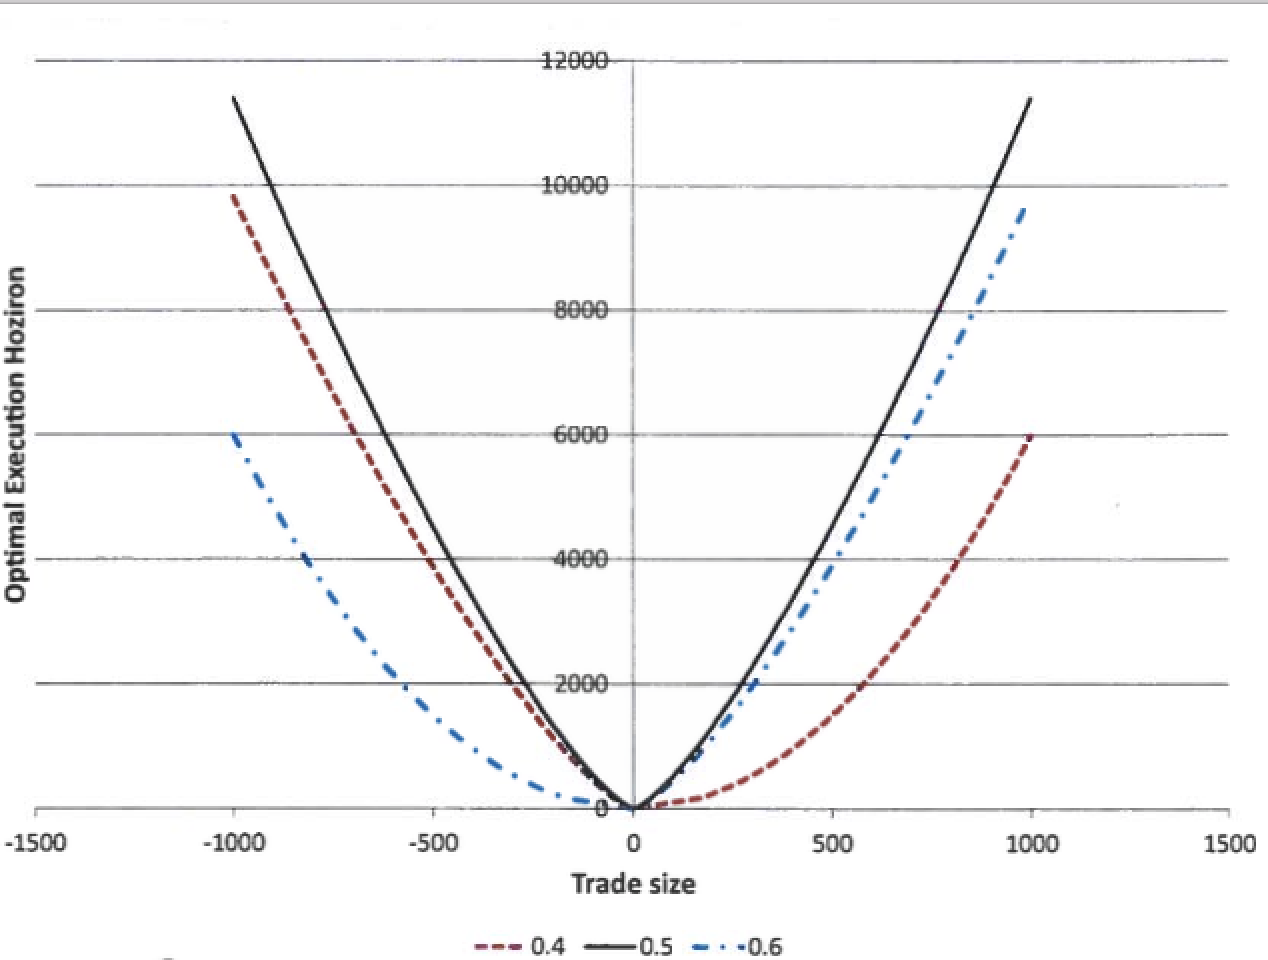
\includegraphics[width=\textwidth]{chapters/chapter7/figures/fig3temp.png}
     \caption{Optimal execution horizons for various order imbalances and trade sizes/sides. Combining alternative trade sizes and sides with our three scenarios ($v^B=0.4$, $v^B=\frac{1}{2}$, $v^B=0.6$) results in the optimal execution horizons displayed in the figure above, $\hat{\sigma}=1,000$, $V_\sigma=10,000$, $m=1,000$, $[\overline{S}-\underline{S}]=10,000$, $\lambda=0.05$ and $\varphi[|m|]$ linear. \label{fig:3temp}}
\end{figure}


\section{Multiple Exchanges:  Smart Order Routing}


In the USA there are over ten lit venues and close to forty dark venues and thus equity markets are highly fragmented. Each venue functions as an electronic limit order book, where orders are prioritized first based on their prices and then at a given price level, according to their time of arrival. Exchanges publish information for each security in real-time and the information can change rapidly due to cancellations. The exchanges may differ with respect to best bid and offer price levels, the market depth at various prices etc. At any point in time, the highest bid and the lowest offer among all exchanges comprise the National Best Bid and Offer (NBBO). The exchanges also differ in their fee structures. Under the maker-taker pricing, exchanges offer rebates to liquidity providers and charge fees to takers of liquidity. These fees can range from $-\$0.001$ to \$0.0030 and since the typical bid-ask spread is \$0.01, the fees and rebates are a fairly significant fraction of the trading costs. Thus market participants must decide where child orders should be sent. It may be expensive to route to all the exchanges and by not routing to the right venue, it is possible to miss liquidity and hence incur greater market impact. Most traders use the smart order routing algorithms with goal to buy or sell the maximum number of shares in the shortest possible time with the least market impact possible. But a key issue is that many of the lit venues have hidden orders (12-45\%). How to estimate the size of the hidden orders and how to make routing decisions in the presence of hidden orders has been a focus of recent research studies.


While exchanges compete along many fronts, for example, payment for order flow, transparency and execution speed, the key variables driving the efficiency are liquidity and price improvement. Thus the design of market structure is considered by market participants and regulators as the key determinant of flow of liquidity. The coexistence of multiple exchanges as mentioned in Parlour and Seppi (2003)~\cite{parlour2003} raises specific questions stated below:

\begin{enumerate}[a)]
\item Do liquidity and trading concentrate in a few exchanges?
\item Do some market designs provide greater liquidity than others?
\item Is the fragmentation of order flow desirable from a policy point of view?
\item What is the constructive role for regulators to enhance liquidity?
\end{enumerate}


Because exchanges operate under rules governing certain market designs, the performance and efficiency issues are related to the types of markets, such as pure limit order and a hybrid market (limit order book plus a specialist). In the hybrid market a specialist can provide supplementary liquidity after a market order has arrived. Parlour and Seppi (2003)~\cite{parlour2003} conclude only under some conditions such as enforcement of time priority, the efficiency is possible. Merely increasing the number of trading venues may result in degradation of market quality, if the enforcement of time priority is not followed; at it might discourage traders from posting the limit orders.


Foucault and Menkveld (2008)~\cite{foumen}consider the effect of fragmentation on two limit order markets. They examine the competition between Euronext and London Stock Exchange (LSE) in the Dutch market. The consolidated limit order book is found to be deeper after entry of the LSE. General conclusions from the above study and others such as Hendershott, Jones and Menkveld (2011)~\cite{hjm} and O'Hara and Ye (2011)~\cite{oye} are that fragmentation of order flows improves the liquidity supply and protecting orders against trade-throughs is important. Thus multiple exchanges are here to stay and smart order routing algorithms that can work well with the increased number of exchanges would be favorably sought by the market participants.


The smart order router (SOR), generally work as follows. A user can customize the use of the strategy by establishing a set of rules in splitting the parent order into child orders and the smart order routers are designed to ensure that the orders are routed to the venue with the best price and the orders are filled according to the trading strategies that may be pre-determined or may be adaptive. To be successful, SORs must be able to handle a variety of trading strategies and multiple venues. In addition they must deal with vast amount of incoming and historical market data. The publicly available information on the SORs used by major traders states that the order placement objective in general is to minimize client all-in shortfall with or without venue fees. The all-in shortfall consists of the shortfall on the filled shares and the cost of the clean-up trade for the unfilled shares. The latter is taken to be an important component of order placement optimization as it enables to quantify the effect of venue differences in fill rates, (see Street Smart, Issue 42, Jan 14, 2011). Other programs used in industry chose to optimize the expected time to execute the client's overall order; expected queue speeds at various venues are predicted from recent trading observations. Small orders tend to be placed in a single venue to minimize the queueing time whereas large orders will be placed in multiple venues to access the maximum liquidity. In this model forecasting trading rates at different venues is crucial for successful implementation of the program. The rates are modeled as a function of lagged rates, thus capturing the momentum, and imbalances between supply and demand sides of the order book. Thus order placement in a fragmented market is not a trivial task.


A recent empirical study by Battalio, Corwin and Jennings (2016)~\cite{} confirms that brokers use both limit and marketable orders to execute trades. Past studies provide evidence that market orders are sent to venues with lower trading costs and the trading fees and rebates generally affect consolidated market depth. Moallemi, Maglaras and Zheng (2012)~\cite{} show that limit orders are submitted to exchanges with high rebates and lower waiting time for execution while market orders are sent to venues that have lower fees and larger posted quote sizes. Cont and Kukanov (2017)~\cite{contk} develop a model that is somewhat more realistic to the current practice by decoupling the `order placement' decision from the scheduling decision and more importantly consider the option of placing limit orders on several exchanges, simultaneously. The model also accounts for the execution risk, the risk of not filling an order. Filling the unfilled portion may be costly and the allocation may shift toward market orders or toward overbooking, that is placing more orders than needed to refill.


To formalize the order placement problem, we assume a size of order $S$ is to be filled in the duration $(0,T)$. The decision is to split this order into a market order $M$ and `$K$' limit orders $L_1,\ldots,L_K$ with the same size to be placed in `$K$' exchanges with queue sizes $Q_1,\ldots,Q_K$ ; thus the order allocation is summarized by the elements of the vector $X=(M,L_1,\ldots,L_K)$ that need to be optimally determined. If order cancellations in the duration $(0,T)$ in exchange `$K$' is represented by $\xi_K$, then the number of shares transacted can be written as 
	\begin{equation}\label{eqn:axe}
	A(X,\xi)= M + \sum_{k=1}^K \left[ (\xi_k - Q_k)_+ - (\xi_k - Q_k - L_k)_+ \right]
	\end{equation}
where the terms in the parenthesis refers to the initial position and the final position of the queue outflows. The execution cost must account for fee ($f$) and rebate structures (discussed in Chapter 6) in each exchange and the cost of adverse selection ($r_k$) and can be stated as follows:
	\begin{equation}\label{eqn:cxe}
	C(X,\xi)= (h+f)M - \sum_{k=1}^K (h+r_k) \left[ (\xi_k - Q_k)_+ - (\xi_k - Q_k - L_k)_+ \right]
	\end{equation}
Here $h$ is one-half of bid-ask spread. 


The cost function in (\ref{eqn:cxe}) can be modified to account for the cost of unfilled limit orders which may be filled through market orders of higher cost or it is possible that the prices have decreased resulting in additional adverse selection cost with penalty ($\lambda_u$) for falling behind and penalty ($\lambda_0$) for exceeding the target; Thus, the execution risk can be written as,
	\begin{equation}\label{eqn:er}
	\text{ER}= \lambda_u (S-A(X,\xi))_+ + \lambda_0 (A(X,\xi)-S)
	\end{equation}
To be more realistic, the market impact function can be considered as follows:
	\begin{equation}\label{eqn:mi}
	\text{MI}= \theta \left[ M + \sum_{k=1}^K L_k + (S-A(X,\xi))_+ \right]
	\end{equation}
The total cost function that includes both implicit and explicit costs can be states as:
	\begin{equation}\label{eqn:vxe}
	V(X,\xi)= C(X,\xi) + \text{ER} + \text{MI}
	\end{equation}
The random variable in (\ref{eqn:vxe}) is $\xi$, the cancellations that occur in various exchanges and the minimization function is $E[V(X,\xi)]$ under some distribution $F$ of $\xi$. Under some reasonable assumptions such as that the trader will not execute more than the target $S$ and market orders in the beginning of the duration $(0,T)$ are less expensive than at the end when unfilled orders are converted to market orders, an optimal solution is shown to exist (see Cont and Kukanov (2017)~\cite{contk} for details).


The analytical solution minimizing $V(X,\xi)$ is not easily tractable due to dimensionality issues. A numerical solution via gradient method is proposed. Random samples of $\xi$ are obtained and averaged to approximate $E(\xi)$. Let $q(X,\xi)= \Delta V(X,\xi)$ be the gradient of $V$. The following iterative algorithm is shown and converges:
	\begin{enumerate}[--]
	\item \textbf{Start with }$\mathbf{X_0}$\textbf{ and for }$\mathbf{n=1,2,\ldots,N}$\textbf{ do}
	\item $\mathbf{X_n=X_{n-1} - \gamma_N g(x_{n-1}, \xi^n)}$
	\item \textbf{End; }$\mathbf{X_N^* = \frac{1}{N} \sum_{n=1}^N X_n}$
	\end{enumerate}
The step size, \small
	\begin{equation}\label{eqn:7gammaN}
	 \gamma_N = \sqrt{k} S \left( N(h+f+\theta+\lambda_u +\lambda_0)^2 _ t + N \sum_{k=1}^K (h+r_k+\theta+\lambda_u+\lambda_0)^2 \right)^{-1/2} 
	\end{equation}
\normalsize can be seen as a function of all the costs associated with the execution of the order.

To summarize, recall that the algorithm needs the following input:
	\begin{enumerate}[--]
	\item Trading Costs: 
		\begin{enumerate}
		\item One half of bid-ask spread ($h$)
		\item Market order fee ($f$)
		\item Effective limit order risks ($r_k$)
		\item Market impact coefficient ($\theta$)
		\item Penalties for overfilling or underfilling ($\lambda_0,\lambda_u$)
		\end{enumerate}
	\item Market Variables: Number of exchanges ($K$) and limit order queues ($Q_k$).
	\item Execution Variables: Time horizon ($T$) and target quantity ($S$).
	\end{enumerate}
While many of these quantities can be estimated using past transactions, the limit order queues ($Q_k$) can the cancellation ($\xi_k$) are to be obtained at the time of execution.


\section{Market Impact Models:  Permanent and Temporary Impacts}


One of the main focuses of Algorithmic Trading is minimizing costs of trade execution. When a large order is executed in the market, it causes market impact (MI), which is commonly defined as the deviation of the post-trade market price from the market price that could have prevailed had the trade not occurred (Fabozzi, Focardi and Kolm (2006)~\cite{ffk}). To alleviate MI and the implied transaction cost (TC), a trader may use an algorithmic trading system to slice a large ``parent'' order into a sequence of ``child'' orders. While a slicing strategy is typically motivated by the liquidity constraint associated with executing a large order in one print, it is usually balanced against the risk and opportunity costs associated with the execution of a sequence of child orders over a longer duration as discussed earlier.


In asset management, with the competitive focus of the industry on cost management and diminishing returns of crowded strategies, understanding and managing MI has become a crucial component of a systematic investment process. For an estimate of its size among the transaction costs that include explicit costs such as brokerage commissions and fees, see Table~\ref{tab:empttrans} from Berkovec and Heidle (2010)~\cite{borkoheidle}. Managing MI has important implications on three aspects of algorithmic trading: pre-trade TC estimation, post-trade TC analysis and the design of optimal trading strategies (Almgren (2008)~\cite{alm2008}).

\begin{table}[!ht]
	\caption{Empirical Transaction Cost Estimates$^1$ \label{tab:empttrans}}	
		\begin{tabular}{|c|c|c|}
		Type & Fixed & Variable\\ \hline
		\hline
		Explicit & Commissions (7.4bp) & Bid-ask spreads (1.9bp)\\ \hline
		& Fees & Taxes\\ \hline
		\hline
		Implicit & & Delay Cost (9.5bp)\\ \hline
		 & & Price Movement Risk \& \\
		 & & Market Impact Costs* (35.6bp)\\ \hline
		 & & Timing Risk \& Opportunity Costs (11.7bp)\\ \hline 
		\end{tabular}
\small *Major Component \\ 1: Readers should note changes in the market that have taken place since these numbers were reported. The commissions are quite expensive for current trading. Most developed markets  have commissions less than 1~bps, while E.M. markets are in the range of 2--5~bps for e-trading. The bid-ask spread makes sense if it is half a spread of liquid U.S. stocks. For other markets, it can be much higher.  \normalsize
\end{table}


The study of price impact dates back to Bagehot (1971)~\cite{} who postulated that the market consists of heterogeneously informed traders. The specialist cannot distinguish between informed and uninformed (liquidity) traders and fixes a spread that can balance the trading cost. The asymmetric information models based on this notion have been extensively studied in finance literature. The traders do convey information and Hasbrouck (1991)~\cite{hasbrouk} provides empirical evidence that the market maker can infer information from the characteristics of the sequence of trades. The seminal work by Kyle (1985)~\cite{kyle1985} and Huberman and Stanzl (2004)~\cite{huberstan} indicate that an order of large size (parent order) must be sliced into a number of small order (child orders) so that the volume per se will not signal informed trading. The hypothesis that time between the trades could convey the information flow (Easley and O'Hara (1992)~\cite{easleyo}) and its impact on price is studied in Dufour and Engle (2000)~\cite{dufour}. Long durations are usually associated with no new news and the variations in trading intensity are taken to be positively correlated with the behavior of the informed traders. \\


\noindent \textbf{Origins of Market Impact:} Most conventional definitions of the MI of a trade equate it with the deviation of the post-trade market price from the market price that would have prevailed had the trade not occurred. Figure~\ref{fig:marketimpt} shows an idealized MI picture of $n$-share sell order from Fabozzi, Focardi and Kolm (2006)~\cite{ffk} but Figure~\ref{fig:detmarketimpt} is augmented to include other information: (1) the state of the order book establishes a pre-trade equilibrium, (2) this equilibrium is disturbed by a market order to sell n shares, (3) as the sell order depletes the bid order book, it obtains an increasingly lower trade price and results in the trade print, and, (4) over time the price gradually moves up back to recover some of the price drop. Accordingly, the difference between (4) and (3) is called temporary impact, whereas the difference between (4) and (1) is called permanent impact. If we are looking to model the MI effect of sequential trades, as shown in Figure~\ref{fig:marketimpt}, the temporary and permanent impact will be superpositions of those of individual trades. The permanent impact is often assumed to be immediate and linear in the parent trade size, and the post-trade equilibrium to be the same for the order of n shares or a sequence of m orders of n/m shares each (Almgren et al. (2005)~\cite{athl}; Fabozzi et al., (2006)~\cite{ffk}). By contrast, the temporary impact is a function of how the ``parent'' trade is split into smaller ``child'' trades.
	\begin{figure}[!ht]
	\centering
	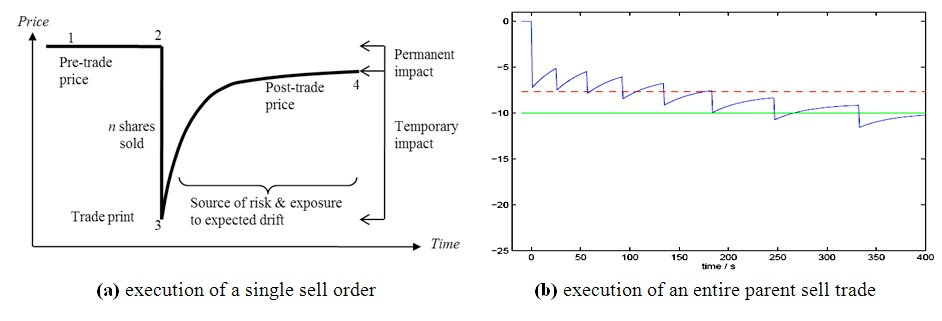
\includegraphics[width=\textwidth]{chapters/chapter7/figures/fig1ab.jpg}
	\caption{Idealized MI Model: single sell trade (left) and entire parent sell trade (right). \label{fig:marketimpt}}
	\end{figure}
The mechanisms responsible for the permanent and temporary impacts have been a subject of significant interest. One common view links price changes accompanying large trades to the information cost and liquidity cost (Chan and Lakonishok (1995)~\cite{chan1995}; Holthausen et al. (1990)~\cite{holthausen1990}) potentially attributed to any transaction. In terms of information cost, the market response to the fact that a market participant has decided to sell (buy) shares of a particular stock could be perceived as conveying new (private) information about the fundamentals of a security (e.g., firm's management, debt conditions) and thus its future prices. Consequently, it results in a permanent price change with no price reversals. In terms of liquidity cost, the market response to the fact that liquidity was removed out of the order book can be perceived as the effect of distorting the liquidity demand/supply equilibrium. The consequence is a temporary price impact that dissipates soon after the trading occurs, at a speed that depends on the market ability to absorb liquidity demand.


Independent of the market microstructure responsible for MI, two central concerns to much theoretical and empirical work are the functional form (shape) of the MI and the key determinants of this form. As seen in Figure~\ref{fig:detmarketimpt}, MI is influenced by trade-related factors (e.g., relative trade size, time of trade), asset-specific factors (e.g., market capitalization, shares outstanding, bid-ask spread) and exchange- and market-related factors (e.g., liquidity, trading volume, institutional features). Models that incorporate these factors tend to be more complex but with better predictive power.
	\begin{figure}[!ht]
	\centering
	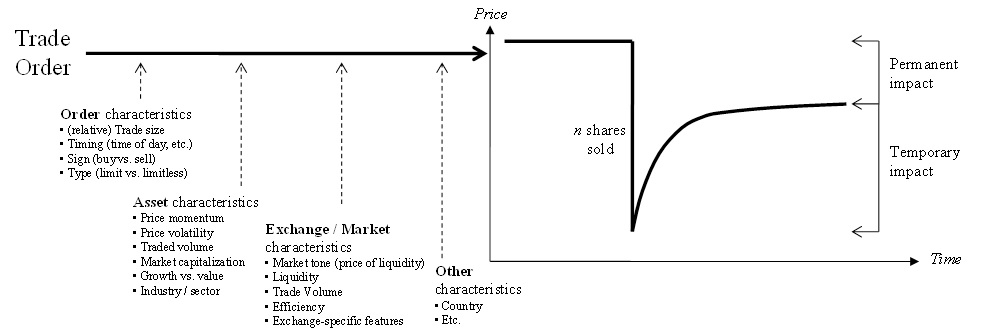
\includegraphics[width=\textwidth]{chapters/chapter7/figures/fig2.jpg}
	\caption{Determinants of Market Impact. \label{fig:detmarketimpt}}
	\end{figure}
Numerous stylized MI models offer some insight into the possible shapes of the permanent and temporary impact functions. Some of these models focus only on the permanent impact, while some models also attempt to capture the effect of temporary impact. \\


\noindent \textbf{Equilibrium Permanent Impact Models:} Models of one class, including Kyle's (1985)~\cite{kyle1985} and Hubberman and Stanzl's (2004)~\cite{huberstan}, rest on the efficient market hypothesis positing that all available information is included in prices. These models use a time-independent framework to establish an equilibrium price after a trade is executed. This means that trades are assumed to have only a permanent price impact (Huberman and Stanzl, 2004, p. 1260)~\cite{huberstan}


Under these settings, Huberman and Stanzl (2004)~\cite{huberstan} show that, if no quasi-arbitrage possibilities exist (to ensure viable markets), the permanent impact must be linear in the trade quantity and symmetric between buys and sells. Linearity in trade size has been established by Kyle (1985)~\cite{kyle1985} as well. In fact, Huberman and Stanzl (2004)~\cite{huberstan} add that ``Nonlinear, time-dependent price-update functions may assume ``chaotic'' shapes without giving rise to price manipulation. Only when additional assumptions are made on the shapes of these functions does the analysis become meaningful.''


Almgren et al. (2005)~\cite{athl} develop a different market impact model, in the context of finding an optimal execution strategy for a large trade [see the discussion of Almgren and Chriss model in Section 7.1.2] that is sliced into several smaller trades. They describe the random process satisfied by the stock price using an arithmetic Brownian process that depends directly on a permanent impact function that is linear in trade size and therefore has no effect on the optimal execution strategy. However, they recognize that if the total number of units traded is sufficiently large, the execution price may steadily change between trades, in part because the supply of liquidity is exhausted at each successive price level. They assume that this effect is short-lived because liquidity returns after each period and a new equilibrium price is established. They model this effect using a temporary price impact function that is non-linear in trade size. They then postulate that both the permanent and temporary impact functions follow power laws based on theirs' and others' empirical results. (Loeb (1983)~\cite{loeb}; Lillo, Farmer and Mantegna (2003)~\cite{farmermantegna}). \\


\noindent \textbf{Hybrid Impact Models:} Models of another class assume that trading agents have zero intelligence (instead of being fully rational) and take random decisions to buy or to sell, but that their action is interpreted by all the others agents as containing some potential information. The mere fact of buying, or selling typically leads to a change of the ask $a$, or bid $b$, price and hence to a change of the midpoint $p=\frac{a+b}{2}$. The new midprice is also expected to follow a random walk (at least for sufficient large times), if it is immediately adopted by all other market participants as the new reference price around which new orders are launched.


Madhavan et al. (1997)~\cite{madhaven1997} develop a price formation model postulating that the (bid-ask) mid price `$p$' changes because of unpredictable public information shocks (news) and microstructure effects that include statistical effects of order flow fluctuations (e.g., autocorrelation) and trading frictions (e.g., asymmetric information, dealer costs). This postulate automatically removes any predictability in the price returns and ensures market efficiency. If all trades have the same volume and the surprise component of the order flow at the $k$th trade is given by $\epsilon_k - \rho \,\epsilon_{k-1}$, where the signs of trades $\epsilon_n$ are generated by a Markov process with correlation $\rho$,\footnote{This means that the expected value of $\epsilon_k$ conditioned on the past only depends on $\epsilon_{k-1}$, given by: $E(\epsilon_k\,|\,\epsilon_{k-1})=\rho\,\epsilon_{k-1}$.}  one writes the following evolution equation for the midprice as:
	\begin{equation}\label{eqn:midpointdelta}
	\Delta p_{k+1}=p_{k+1}-p_k=\theta[\epsilon_k - \rho \epsilon_{k-1}]+\eta_k
	\end{equation}
where $\eta$ is the shock component and the constant $\theta$ measures the size of trade impact. Empirical estimation of their model are not aimed at investigating the shape of impact functions.\footnote{First, both information flows and trading frictions are important factors in explaining intraday price volatility in individual stocks. Second, information asymmetry decreases steadily throughout the day, however, dealer costs increase over the day (possibly reflecting the costs of carrying inventory overnight) so that bid-ask spreads exhibit the U-shaped pattern commonly noted in previous research studies.}


Others extend the model of Madhavan et al.~(1997) to gain insight into the shape of impact functions.  Bouchaud et al. (2009)~\cite{bouchaud2009} use (\ref{eqn:midpointdelta}) to compute several important quantities. Principally, they write the lagged return impact function (for time points $n$ and $n+l$), denoted $R_l$, as:
	\begin{equation}\label{eqn:rlittlel}
	R_l = p_{n+l}-p_n = \theta \sum_{j=n}^{n+l-1}[\epsilon_j - \rho \epsilon_{j-1}]+ \sum_{j=n}^{n+l-1}\eta_j
	\end{equation}
and then show that the lagged impact function is constant and equal to:
	\begin{equation}\label{eqn:rlittlel2}
	R_l = \theta (1-\rho^2), \forall l
	\end{equation}
Now define the ``bare'' impact of a single trade taken at time $l$, denoted $G_0(l)$, which measures the influence of a trade at time $n-l$ on the bid-ask midprice at time $n$. Written in terms of $G_0(l)$, the midpoint process is expressed as:
	\begin{equation}\label{eqn:plittlen}
	p_n = \sum_{j=-\infty}^{n-1}G_0(n-j-1)\,\epsilon_j + \sum_{j=-\infty}^{n-1}\eta_j
	\end{equation}
Then it can be shown that $G_0(0) = \theta$ and $G_0(l) = \theta(l-\rho)$ for $l>0$. Bouchaud et al. (2009)~\cite{bouchaud2009} also observe that ``The part $\theta \rho$ of the impact instantaneously decays to zero after the first trade, whereas the rest of the impact is permanent. The instantaneous drop of part of the impact compensates the sign correlation of the trades.''


Bouchaud et al. (2004)~\cite{bouchaud2004} have developed an earlier price evolution model, similar to (\ref{eqn:rlittlel}), where the price at time $n$ is written as a sum over all past trades of the impact of one given trade propagated up to time $n$:
	\begin{equation}\label{eqn:anotherplittlen}
	p_n = \sum_{n'<n} G_0(n-n')\,\epsilon_{n'} \ln{V_{n'}} + \sum_{n'<n} \eta_{n'}
	\end{equation}
where $V_n$ denotes the volume of a trade at time n and $G_0()$ is assumed to be a fixed non-random function that only depends on time differences. The $\eta_n's$ are also random variables, assumed to be independent from $\epsilon_n$, and are used to model all sources of price changes not described by the direct impact of the trades. The authors then consider constraints imposed on the shape of response function, $G_0$, by three empirical results they discuss: (a) the midprice price process is close to being purely diffusive, even at the trade-by-trade level; (b) the temporal structure of the impact function first increases and reaches a maximum after some number (100 to 1000) of trades, before decreasing back with a rather limited overall variation; and the sign of the trades shows surprisingly long-range, power-law correlations. These empirical results are reconciled with (\ref{eqn:anotherplittlen}) by assuming that the response function $G_0()$ must instead also decay as a power-law in time, with an exponent precisely tuned to ensure simultaneously that prices are nearly diffusive and that the response function is nearly constant. Gatheral (2010)~\cite{gatheral}, assuming that the trading costs should be non-negative, demonstrates that the exponential decay of market impact is compatible only when the market impact is taken to be linear. Thus the debate on the functional form of MI is ongoing. 


It has been noted that the models developed to study market impact generally do not consider situations that may arise from strategies where price impact may depend upon the state of the order book. The second generation models consider the behavior of the limit order book. Hautsch and Huang (2012)~\cite{hauthuang} consider a time-aggregated model. The activities in the book are captured in Table~\ref{tab:vardef} and the market depth is kept to the three best quotes on both sides of the market.
	\begin{table}[!ht]
	\centering
	\caption{Model (\ref{eqn:7dy}) Variable Definitions \label{tab:vardef}}
	\begin{tabular}{ll}
	Variable & Description \\ \hline
	$p_t^a$ & Logarithm of the best ask after the $t$-th event. \\
	$p_t^b$ & Logarithm of the best bid after the $t$-th event. \\
	$v_t^{a,l}$ & Logarithm of the market depth at the $l$-th best ask after the $t$-th event. \\
	$v_t^{b,l}$ & Logarithm of market depth at the $l$-th best bid after the $t$-th event. \\
	$\text{BUY}_t$ & Dummy equal to one if the $t$-th event is a buyer-initiated trade. \\
	$\text{SELL}_t$ & Dummy equal to one if the $t$-th event is a seller-initiated trade. 
	\end{tabular} 
	\end{table}
Let $Y_t$ be a $K$-dimensional listing the variables in Table~\ref{tab:vardef}; the co-integration model in Chapter 2 is fit for the data:
	\begin{equation} \label{eqn:7dy}
	\Delta Y_t = \mu + \alpha \beta' y_{t-1} + \sum_{t=1}^{p-1} \Gamma_i \Delta Y_{t-i} + u_t
	\end{equation}
The co-integrating $(K \times r)$ matrix, $\beta$ has first two columns restricted to have entries as zeros except for buy and sell indicators. To study the market impact, the model is written in the reduced-form to capture the impulse-response coefficients as:
	\begin{equation}\label{eqn:7largeyt}
	Y_t = \mu + \sum_{i=1}^p A_i Y_{t-i} + U_t
	\end{equation}
where $A_1=I_k+\alpha\beta' + \Gamma_1$, $A_i=\Gamma_i - \Gamma_{i-1}$ for $1<i<p$ and $A_p= -\Gamma_{p-1}$. The $\text{VAR}(p)$ model in (\ref{eqn:7largeyt}) can then be written in the form of $\text{VAR}(1)$ as 
	\begin{equation}\label{eqn:starlargeyt}
	Y_t^*= \mu^* + A^* Y_{t-1} + U_t^*
	\end{equation}
where $\mu^*=(\mu',0',\ldots,0')'$, $Y_t^*=[Y_t',Y_{t-1}',\ldots,Y_{t-p+1}']$, $U_t^*=[U_t',0',\ldots,0']'$ and $A^*=\renewcommand\arraystretch{1.3} \mleft[ \begin{array}{c|c} A_1\cdots A_{p-1} & A_p \\ \hline I_{K(p-1)} & 0 \end{array} \mright]$. It can be shown that 
	\begin{equation}\label{eqn:7anotherlargeyt}
	Y_t= JM_t + \sum_{i=0}^{t-1} JA^i J' U_{t-i}
	\end{equation}
where $J=[I_k,0,\cdots,0]$ is a $k\times kp$ selection matrix and $M_t= A^{*t} Y_0^* + \sum_{i=0}^t A^{*i}U_{t-i}^*$.

Recall that the market impact measures the impact of current trade on the future trades; it is measured by the impulse response function
	\begin{equation}\label{eqn:impulserep}
	f(h,\delta_h) = E[y_{t+h}\,|\, y_t+\delta_y,t_{t-1},\cdots] - E[y_{t+h} \,|\, y_t,y_{t-i},\cdots] = JA^{*h} J' \delta_y
	\end{equation}
where $\delta_y$ is the change to $Y_t$, due to the current trade. The long-run effect, $f(\delta_y)=C \delta_y$, where $C=\beta_\perp(\alpha_\perp'(I_K - \sum_{i=1}^{p-1} \Gamma_i ) \beta_\perp )^{-1} \alpha_\perp'$. Here $\alpha_\perp$ and $\beta_\perp$ are orthogonal to $\alpha$ and $\beta$ in (\ref{eqn:7dy}).


Hautsch and Huang (2012)~\cite{hauthuang} estimate the market impact using the data from Euronext, Amsterdam for heavily traded stocks. The main findings are, besides the existence of co-integrating relationships between quotes and depths, limit orders have long-term effects on quotes, the price movement is influenced by the order size and the decrease of spreads after the arrival of a limit order is reverted back asymmetrically soon after. The between-stock variations in market impact are shown to be related to trading frequency of the stocks. 


Cont, Kukanov and Stoikov (2014)~\cite{contkulst} consider the dynamics of market liquidity that is a function of limit orders, market orders and cancellations to model the price impact function. The outstanding limit orders provide a measure of depth in the market on both buy and sell sides and thus also provide a measure of order flow imbalance (OFI).


By setting the number of shares (depth) or price levels beyond the best bid and ask is equal to $D$, define the price change in the interval $(t_{k-1},t_k)$ as,
	\begin{equation}\label{eqn:doubleeq}
	\begin{split}
	\Delta P_k^b&= \delta \left[ \dfrac{L_k^b - C_k^b - M_k^s}{D} \right] \\
	\Delta P_k^s&= -\delta \left[\dfrac{L_k^s-C_k^s-M_k^b}{D}\right]
	\end{split}
	\end{equation}
where $L_k^i$, $C_k^i$ and $M_k^i$ for $i=b,s$ denote arrival of the limit orders, cancellations and market orders in the defined interval. Here $\delta$ is the tick size. If $P_k=\dfrac{P_k^b+P_k^s}{2\delta}$, that is mid-price normalized by tick size, for any $s$nd-interval, $(t_{k-1,i},t_{k,i})$, it is postulated that
	\begin{equation}\label{eqn:postulated}
	\Delta P_{k,i} = \beta_i \text{OFI}_{k,i} + \Eulerconst_{k,i}
	\end{equation}
where $\text{OFI}_k=(L_k^b-C_k^b-M_k^s)-(L_k^s-C_k^s-M_k^b)$ and $\Delta P_k=\frac{\text{OFI}_k}{2D}+\epsilon_k$. Here it is important to note that `$\beta_i$' is taken to be price impact coefficient and is taken to be inversely proportional to market depth:
	\begin{equation}\label{eqn:7betai}
	\beta_i=\dfrac{C}{D_i^\lambda} + v_i
	\end{equation}
The models in (\ref{eqn:postulated}) and (\ref{eqn:7betai}) can be regarded to represent instantaneous price impact. The model as it can be seen from the set-up assumes that all activities in the limit order book have an average linear impact, $\beta_i$, in the $i$th interval. 


Cont et al. (2014)~\cite{contkulst} using the TAQ data for a month in 2010 for fifty stocks estimate the model in (\ref{eqn:postulated}) over ten-second intervals. The model is generally confirmed by the data with $\hat{\beta}_i$ is significant in most of the samples and $\hat{\alpha}_i$ is only significant in less than twenty percent of the samples. It must be noted that there is a significant number of trades posted gets cancelled within a few seconds of submission. Various theories that are postulated (see Hasbrook and Saar (2009)~\cite{habbrooksaar}) are yet to be fully empirically tested. Hence instead of using OFI, trade imbalance $(\text{TF}_k=M_k^b-M_k^s)$ is used in equation (\ref{eqn:postulated}). Results are still reasonable, but not as strong as using OFI in the model. Finally the relationship between $\hat{\beta}_i$ and $D_i$ (price impact coefficient and depth) is studied; the results indicate for model (\ref{eqn:7betai}), $\hat{C} \sim 0.5$ and $\hat{\lambda} \sim 1$. Some interesting conclusions that could be useful for trading are drawn. The impact coefficient varies more with the amount of liquidity provision (OFI) than the trade imbalance (TI). It can be also used to monitor adverse selection. If a limit order is filled after a positive OFI, price is likely to go up and for a limit sell order, a positive change would imply that the order was executed at a loss. These conclusions need to be firmed up with further studies in this area. \\


\noindent\textbf{Determinants of Empirical relationship:} A key aspect of MI modeling is to provide information about expected pre-trade costs. The studies that have been reviewed on empirical analysis thus far can help us to understand how the price formation and the market impact function evolve during a trading period. But most clients who want to trade large quantities of equities want to know the trading costs apriori. Here we review the relevant studies and augment with our own research in this area. First we review the factors that are found to influence these costs in block trades. Although block trades differ in fundamental ways to algorithmic, they can be treated as all equivalent to a parent trade except that no splitting into child orders occurs.


\begin{itemize}
\item \textbf{Trade Size.} Many studies observe that the (relative) size of trades positively relates to the magnitude of MI (Keim and Madhavan (1996)~\cite{madhavan}), consistent with the prediction of stylized model (Kyle (1985)\cite{kyle1985}; Huberman and Stanzl (2004)~\cite{huberstan}).

\item \textbf{Market Capitalization.} Keim and Madhavan (1996)~\cite{keim1996}find that the asymmetry of trading costs between buys and sells is more pronounced among smaller stocks. This is consistent with what is broadly known to be the effects of market capitalization on MI (Lillo et al. (2003)~\cite{farmermantegna}; Chan and Lakonishok (1997)~\cite{chan1997}). From a practical point of view, market cap itself may not be a true factor but it can be a proxy for some liquidity characteristics. 

\item \textbf{Price Volatility.} Price volatility has been found to be positively related to MI (Chiyachantana et al. (2004)~\cite{chiya2004}). One explanation is that elevated volatility is associated with greater dispersion in beliefs, with risk averse traders less inclined to participate in markets, thereby resulting in greater price concessions or MI (Domowitz et al. (2001)~\cite{domo2001})

\item \textbf{Trading Activity.} Dufour and Engle (2000, p. 2467)~\cite{dufour} find that the price impact of trades increases as the time duration between transactions decreases, and more broadly that the price impact is especially large due to increased trading activity, as measured by high trading rates. In their view, ``times when markets are most active are times when there is an increased presence of informed traders; we interpret such markets as having reduced liquidity.'' Likewise, Yang (2011, p. 91)~\cite{yang2011} finds that ``a trade shortly after the previous trade results in higher price impact than one after a long period.'' He also offers ``evidence that increased trading activity (as measured by short durations between trades) is associated with larger price impact, therefore implying a higher degree of information-based trading.''

\item \textbf{Time of Day.} It is reported that the MI for buy trades decreases as time passes during the day, with the highest impact in the first trading hours (Frino et al. (2007)~\cite{frino}).
\end{itemize}


We will now summarize briefly the models that are used in the industry. For many years, traders have used the simple sigma-root-liquidity model described for example by Grinold and Kahn (1994)~\cite{grin2000}. The model takes the form,
	\begin{equation}\label{eqn:spreadcost}
	\Delta P - \text{Spread Cost} = \alpha\cdot\sigma\sqrt{\frac{X}{V}}
	\end{equation}
where $X$ is the size of the parent order, $V$ is the average daily volume and `$\sigma$' is the volatility of the stock. Thus the relative size (RS), $\frac{X}{V}$ is the key factor in the pre-trade cost estimation and the impact is proportional to volatility. The square root of relative size is expected because risk capital should be proportional to the square-root of the holding period. In Toth et al. (2011)~\cite{toth2011anomalous}, the authors present an argument that if latent supply and demand are linear in price over some plausible range of prices, which is a reasonable assumption, market impact should be square-root.


The square-root formula as stated in (\ref{eqn:spreadcost}) refers only to the size of the trade relative to daily volume. It does not refer to for example, the rate if trading, how the trade is executed and the market capitalization of the stock. If the trading is quite aggressive, the square-root formula tends to break down. Moro et al (2009)~\cite{moro2009market} observe that the price path during the execution follows a power law:
	\begin{equation}\label{eqn:ptalpha}
	p_t - p_0 = \alpha\cdot({\frac{t}{T}})^{2/3}
	\end{equation}
where $T$ is the duration of the parent-order. Immediately after completion of a parent-order, the price begins to revert. Other models used in industry are mostly functions of the determinants identified above. \\


\noindent\textbf{Select Empirical Studies:} While there is some discussion about the theoretical models for market impact, published studies based on large scale data are somewhat rare especially when it comes to models useful for pre-trade cost estimation, Almgren et al (2005)~\cite{athl} took US stock trade orders processed by Citigroup for Dec 2001 - June 2003 and estimated a model of the market impact as given in Table~\ref{tab:costimpact}. For two select stocks, IBM and DB, the power law model for market impact are estimated. The temporary impact is defined as $\widetilde{p}_k - p_{k-1}$, for $k^{th}$ execution. The model depends on relative size, inverse turnover ratio, which is the number of the shares outstanding to average daily volume and the volatility.


While the square root formula in (\ref{eqn:spreadcost}) is quite robust and holds even beyond equity markets, recent empirical studies confirm the need for more general power law functions; the quotient of $\text{RS}=\frac{X}{V}$ varies depending on other factors that get included in the model (refer to the estimates in Table~\ref{tab:costimpact} for RS). Zarinelli, Treccani, Farmer and Lillo (2015)~\cite{zar} show that logarithmic functional form fits the data better for the large order data that they consider. 


\begin{table}[!ht]
\caption{Example of impact costs (Almgren et al. (2005)~\cite{athl} \label{tab:costimpact}}
\begin{tabular}{cccc}
 & & IBM & DRI \\ \hline
Average daily volume & $V$ & 6.561~m & 1.929m~ \\
Shares outstanding & $\theta$ & 1728~m & 168~m \\
Inverse turnover & $\theta/V$ & 263 & 87 \\
Daily volatility (\%) & $\sigma$ &1.57 & 2.26 \\
Normalised trade size & $X/V$ & 0.1 & 0.1 \\ \hline
Normalised permanent & $l/\sigma$ & 0.126 & 0.096 \\
Perm. price impact (bp) & $l$ & 20 & 22 \\ \hline
Trade duration (days) & $T$ & 0.1 \hspace{0.2cm} 0.2 \hspace{0.2cm} 0.5 & 0.1 \hspace{0.2cm}0.2 \hspace{0.2cm} 0.5\\
Normalised temporary & $K/\sigma$ & 0.142 \hspace{0.2cm} 0.094 \hspace{0.2cm}0.054 & 0.142 \hspace{0.2cm} 0.094 \hspace{0.2cm} 0.054 \\
Temp. Impact cost (bp) & $K$ & 22 \hspace{0.2cm} 15 \hspace{0.2cm} 8 & 32  \hspace{0.2cm}21\hspace{0.2cm} 12 \\ \hline
Realised cost (bp) & $J$ & 32 \hspace{0.2cm} 25 \hspace{0.2cm} 18 & 43 \hspace{0.2cm}32 \hspace{0.2cm} 23
\end{tabular}
\small Note: examples of permanent and temporary impact costs are shown, for a purchase of 10\% of the day's average volume, in two different large-cap stocks. The permanent cost is independent of time of execution. The temporary cost depends on the time, but across different assets it is the same fraction of daily volatility (from Almgren et al. (2005)~\cite{athl}). \normalsize
\end{table}


Limited access to broker-proprietary algorithmic trading data has stifled detailed academic inquiry in this area. While the impact of algorithmic trading is extensively discussed in the finance literature, formal empirical results are rare. The few exceptions we are aware of are: Engle et al (2012)~\cite{engle2012}, who use proprietary algorithmic trading data from Morgan Stanley to study the risk-return tradeoff associated with increasing the number of child trades and duration of parent trade; Domowitz and Yegerman(2005)~\cite{doye}, who use ITG's Transaction Cost Analysis Peer Group Database to compare execution costs for a set of 40 buy-side clients; and Hendershott and Riordan (2011)~\cite{hernderrio}, who use algorithmic trading data from firms listed on the Deutsche Boerse DAX to measure the contribution of algorithmic trading to price discovery. A few academic studies resort to using proxies based on publicly-available TAQ data. Two examples are: Hendershott et al. (2011)~\cite{hender2011}, who use NYSE electronic message traffic data as a proxy for algorithmic liquidity supply to study how algorithmic trading effects liquidity and bid-ask spreads; and Chaboud et al. (2014)~\cite{chaboud}, who use FX quote data (highest bid and lowest ask) from an electronic limit order book platform called EBS to construct mid-quote series for studying the effect of algorithmic trading on FX rates' volatility. The use of mid-point prices, in the lack of actual arrival price and completion price for a parent trade, has been criticized for failing to capture the possible asymmetry of the bid and ask price impacts of trading, which has been observed to exist for block trades. In any event, none of these studies deals with the estimation of MI models per-se.


Velu, Gretchika, Benaroch, Nehren and Kuber (2015)~\cite{unpub} address these issues using a large algorithmic trading dataset provided by J.P. Morgan Chase. The data contain ``parent'' algorithmic executions, including the initial arrival price and fill price as well as the child trades' average fill price (computed as the share-weighted average executing price of the child orders). The algorithmic executions are generated using Volume Weighted Average Price (VWAP) and Percent of Volume (POV) strategies.Recall the volume weighted average price (VWAP) strategy schedules to trade some constant percentage of the expected market volume regularly throughout the day, where the proportion traded is adjusted based on historical market volume profiles and the predict volume. Hence, in VWAP, the trading schedule is predetermined based on a prediction of the daily market volume distribution, although the timing of executions may be randomized so as to make the trading pattern less predictable. By contrast, the percent of volume (POV) strategy trades a fixed percentage of the current market volume where the trading schedule is dynamically determined based on a historical analysis of volume profiles used to anticipate trading volumes. Unlike implementation shortfall strategies, VWAP and POV do not explicitly take into account the expected MI in generating their algorithmic executions. Moreover, although firms typically implement proprietary versions of these strategies with parameters reflecting their experience and clients' profiles, VWAP and POV nonetheless generate relatively standardized algorithmic executions. In other words, from the perspective of MI, these two strategies can be safely considered ``plain vanilla'' in the sense that firm-to-firm differences in their behavior and performance are too insignificant. The measures employed, therefore, do not depend on any unique traits of the strategies. The unique aspect of the data is that if the meta order is on the buy side or sell side is explicitly provided. 


The dataset allows us to study the effect of parent characteristics on the market impact and the implied transaction cost (TC). Specifically, we estimate the parameters of a family of power-law models, investigate the explanatory power of different determinants of market impact and TC, and develop insights useable for pre-trade cost estimation. Our model estimation effort is informed by existing stylized market impact models and empirical findings about the market impact of block trades. These stylized models are reviewed earlier in this section. In addition to studying the effects of buy and sell trades, order size, price volatility and market cap, we examine the effect of the number of child trades and duration of the parent trade. Lastly, we also summarize two extensions of our model estimation effort that pertain to the effect of the bid-ask spread on market impact and to the market impact of ETFs traded via algorithmic trading.


This study has some important findings. A central novel insight that emerges from the analysis is that market impact can be substantially decreased by reducing the number of child order trades. There could be several explanations, but a simple plausible one is that reducing the number of child trades reduces the information leakage about trading intentions. This explanation is in line with the main premise of Farmer et al. (2012)~\cite{farmer2012} that, in an efficient market, market impact is determined by the information that is disseminated through trades. It is also consistent with studies showing that the price impact is larger as the duration between trades decreases and there is increased trading activity (Dufour and Engle 2000~\cite{dufour}; Yang 2011~\cite{yang2011}), and that the number of trades may drive prices more than the actual trade size (Jones et al. 1994~\cite{jones1994}).


Another finding is the nuanced difference in market impact and TC that is related to buy and sell trades. On the overall level, this difference is statistically significant, and this presumably contradicts the buy-sell market impact asymmetry commonly reported for block trades. However, a deeper examination reveals a more nuanced difference between buy and sell trades. Visual inspection of the TC vs. trades' relative size and the TC vs stocks market cap shows that in some sub-ranges there is a difference between buys and sells. After dividing trades into 24 bins based on their relative size and testing the TC difference within each bin we observe that the difference is statistically significant in six bins; six out of 24 exceeds the proportion expected when testing multiple hypotheses at a 5\% significance level. Consequently, separate market impact and TC models for buy and the sell trades are estimated, and observed the following about the difference between the coefficients of buys and sells. This difference is significant in models containing a subset of the explanatory factors (e.g., relative size alone, or relative size and volatility), but it is within a two standard errors threshold in models containing all the factors. Our findings notwithstanding, it is necessary to investigate further whether the underlying causes may be linked to the specifics of trade flow, the logic behind many of the trading algorithms.


It is important to mention two caveats . One relates to the role of permanent versus temporary impact in our analysis. The data set does not contain information about the price dynamics after the completion of the parent trades, that is, only completion price for the last child order is available. Therefore, it was not possible to determine what portion of the measured market impact is permanent and what portion of it is temporary. Another caveat relates to the high variability in the data. To obtain a better signal out of the noisy data, the data was smoothed through binning and extraction of key descriptives. The models are based on these descriptives. Nevertheless, for robustness testing all models were estimated using the raw unsmoothed data and the results are qualitatively similar, albeit the $R$-square values are understandably much lower. \\


\noindent\textbf{Empirical Details: } The market impact is modeled as a non-linear function of several stock-related and trade-related factors. The power law form is generally recommended for non-linear shape. The data analyzed in Velu et al. (2015)~\cite{unpub} consists of over 250,000 parent orders fully executed over a one-year period, Oct 1, 2009--Sept 30, 2010. All trades were completed within a single trading day. Each parent trade was sliced into multiple child trades; each child trade was executed in one or several partial fills. Only parent trades executed through widely used VWAP (volume-weighted average price) or POV (percent of volume) strategies (Brandes et al. (2007)~\cite{brandes2007}). This ensures that the participation rate is well-defined and stays roughly constant over the duration of the parent trade. We define 
	\small
	\[
	\text{Market Impact (MI) in bps }= \text{side } \cdot \left(\dfrac{\text{\small Completion Price} - \text{\small Arrival Price}}{\text{\small Arrival Price}}\right) \cdot 10000
	\]
	\[
	\text{Transaction Cost (TC) in bps}= \text{side } \cdot \left(\dfrac{\text{\small Average filled Price }-\text{ \small Arrival Price}}{\text{\small Arrival Price}} \right) \cdot 10000
	\]
\noindent \normalsize where the arrival price is the price when the first child order is executed and completion price is the price when the last child order is executed. Every trade in this data is explicitly identified as buy or sell. This contrasts with studies that use TAQ data that do not have the same explicit identification. Using Lee and Ready (1991)~\cite{leeready} heuristic rule to determine the trade direction can be sometimes inaccurate (Asquith, Oman and Safaya (2011)~\cite{asquith2010} and Chakrabarty, Moulton and Shkilko (2012)~\cite{chakrabarty2012short}). To make the analysis robust, we binned the explanatory variables and obtained smoothed averages; the analysis is based on binned data.


Results start with a visual inspection of the relationships. The graphs clearly indicate that the relationship between MI and RS is non-linear, and it remains non-linear with binning of other factors as well. The relationship between MI and relative size is monotonic till the relative size reaches 20\% or so (Figure~\ref{fig:oneoffive}).Trades with longer durations clearly have a lower MI (Figure~\ref{fig:twooffive}). Trades for higher volatility stocks, too, can be read to have a higher MI (Figure~\ref{fig:threeoffive}). Trades on larger market cap stocks have a smaller MI (Figure~\ref{fig:fouroffive}). Lastly, MI becomes higher as the number of child trades increases (Figure~\ref{fig:fiveoffive}). This last relationship is important and deserves special attention particularly when designing execution strategies. There is a clear trade-of between low ``immediate'' liquidity impact of small child orders and long term information leverage of the parent order level when hitting the market too frequently. But the power law model is more general and can accommodate interaction effects as well. These graphs for various factors besides RS can be collapsed into a master curve, with appropriate normalization, as given in Lillo et al. (2003)~\cite{farmermantegna}.
	
	
	\begin{figure}[!ht]
	\centering
	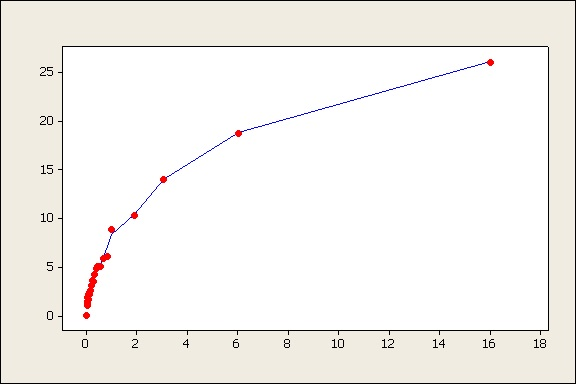
\includegraphics[width=\textwidth]{chapters/chapter7/figures/fig3.jpg}
	\caption{MI vs. RS. \label{fig:oneoffive}}
	\end{figure}

	\begin{figure}
	\centering
	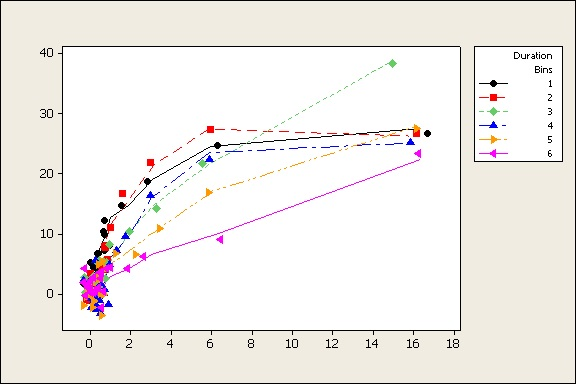
\includegraphics[width=\textwidth]{chapters/chapter7/figures/fig4.jpg}
	\caption{MI vs. RS and Duration. \label{fig:twooffive}}
	\end{figure}

	\begin{figure}
	\centering
	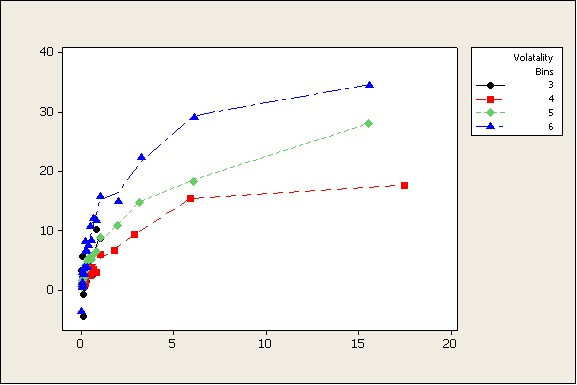
\includegraphics[width=\textwidth]{chapters/chapter7/figures/fig5.jpg}
	\caption{MI vs. RS and Volatility. \label{fig:threeoffive}}
	\end{figure}

	\begin{figure}
	\centering
	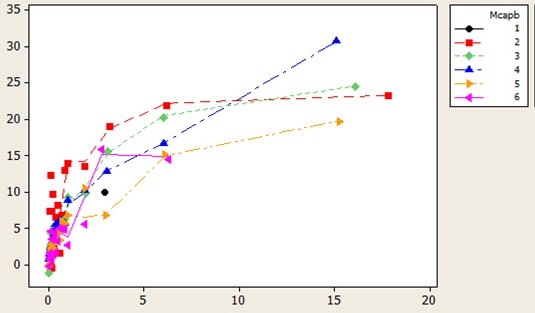
\includegraphics[width=\textwidth]{chapters/chapter7/figures/fig6.jpg}
	\caption{MI vs. RS and Market Cap. \label{fig:fouroffive}}
	\end{figure}

	\begin{figure}
	\centering
	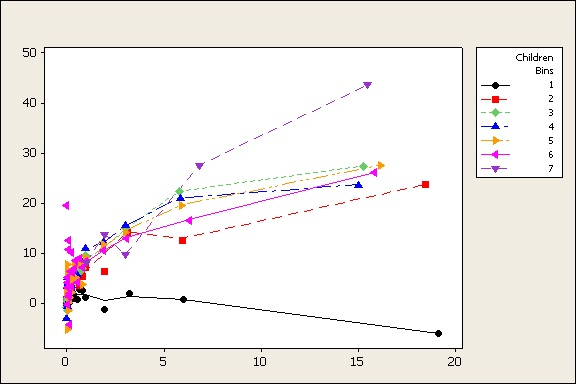
\includegraphics[width=\textwidth]{chapters/chapter7/figures/fig7.jpg}
	\caption{MI vs. RS and No. of Children. \label{fig:fiveoffive}}
	\end{figure}


Table~\ref{fig:marketimpt} shows the results of power-law models ; the standard errors are shown in parentheses below the estimated regression coefficients. All coefficients in the models presented in Table~\ref{fig:marketimpt} are statistically significant. This is consistent with Almgren et al. (2005)~\cite{athl}, except that in their model the market-cap-to-volume ratio is not significant. It should be noted that the values of $R$-square are significantly higher than other published studies, mainly due to binning and smoothing. The response variable is not an individual parent trade cost, but rather the average cost for trades in a bin representing a combination of various levels of predictors. Thus, the models developed here are intended to predict the average MI for a combination of predictors.


\begin{table}[!ht]
\caption{Response Variable is MI (bps) ($\hat{\sigma}^2=225, n=2,$ 211 bins)}
\begin{tabular}{|c|c|c|c|c|c|c|}
Predictor & Model 1& Model 2 & Model 3 & Model 4 & Model 5 & Model 6* \\ \hline
Rel. Size & 0.53 & 0.51 & 0.56 & 0.63 & 0.43 & \\
	& (0.02) & (0.02) & (0.02) & (0.02) & (0.02) & \\
Volatility & & 1.12 & 0.92 & 1.17 & 0.53 & \\
	& & (0.09) & (0.09) & (0.11) & (0.1) & \\
Duration	& & & $-0.24$ & $-0.25$ & $-0.47$ & $-0.27$ \\
	& & & (0.02) & (0.02) & (0.3) & (0.1) \\
Market Cap & & & & $-0.09$ & $-0.12$ & $-0.04$ \\
	& & & & (0.02) & (0.02) & (0.07) \\
No. of Children & & & & & 0.53 & 0.55 \\
	& & & & & (0.04) & (0.16) \\
Constant & 9.6 & 19.6 & 15.9 & 9.4 & 2.7 & 1.3 \\
	& (0.34) & (1.07) & (0.9) & (1.3) & (0.46) & (1.3) \\
\hline
$\hat{\sigma}_{\text{error}}^2$ & 143 & 136 & 125 & 124 & 114 & N/A \\
$R^2$ & 0.37 & 0.40 & 0.45 & 0.45 & 0.50 & 0.03 \\
\end{tabular}
\small*Response Variable$ = \frac{\text{MI}(\text{bps})}{(\text{Vol})(\text{RS})^0.6}$\normalsize
\end{table}


Several relevant observations can be made about the coefficients in the estimated models. For example, Model 3, which is traditionally well cited in the literature, can be written as:
	\[
	\text{MI(bps)}= 15.9\cdot\sigma^{0.92}\cdot(RS)^{0.56}\cdot T^{-0.24}
	\]
Note that the volatility coefficient is approximately `one' and the coefficient of RS is about 0.5 has indeed been observed in the literature. It is consistent with the folklore that it takes one day's volatility to trade one day's volume. The duration effect is also consistent as most of the parent trading occurs in less than two hours in the data set, not always in real life. This has led us to consider an additional model where $\frac{MI(bps)}{(Vol)(RS)^{0.6}}$ is used as a normalized response variable. This variable can be taken as the multiplicative residual term of  Model (2) in Table~\ref{fig:marketimpt}.The regression results of this variable on other variables are given under Model (6*). Two observations can be made: the duration and the number of child trades are still significant factors. However. The increase in $R$-square is somewhat smaller than the unrestricted versions of the same model, labeled as Model (5) in Table~\ref{fig:marketimpt}.


Other key findings can be summarized as follows:

\begin{itemize}
\item Relative size and volatility consistently exhibit positive influences on MI; their impact varies depending on other factors in the model.

\item Duration has an inverse effect. Its use in the model must be carefully calibrated as the execution of parent trades using child trades can be highly concentrated.

\item Stocks with higher market capitalizations tend to have smaller price impact for the same relative size.

\item The number of child trades, which is usually determined by the trading algorithm, does reveal a positive effect on MI.
\end{itemize}

There are several practical considerations that may limit the use of these model for pre-trade cost estimation. These challenges in MI calibration is due to the following facts:
	\begin{enumerate}[--]
	\item Not enough data for certain combinations of the factors involved.
	
	\item MI is a noisy measure which is hard to calibrate ex-post.
	
	\item Sometimes, market moves at a much larger magnitude than MI.
	
	\item Use of raw data results in a poor predictive models; thus a need for aggregation. But aggregation obviously ignores the wide variation within the aggregated unit. 
	\end{enumerate}

\section{Microstructure Noise Models for Multiple Stocks:  Issues of Synchronizations, etc.}
\section{Simultaneous Execution Algorithms for Multiple Instruments}
\section{A Stochastic Adaptive Control Approach to Optimal Execution}
\section{Role of Market Makers in Limit Order Markets}
\section{Open Issues}
\section{Supplements and Problems} 	